% Provenance (never printed): old terminale S material on the continental crust
% (granitic composition, thickness, density, age; roots and isostasy). Thickness
% from Christensen-Mooney 1995 and Cogley 1984 (CRUST1.0 dropped: no licence,
% Sync 1); ocean-floor ages from figdata/grade-12/crust_ages.py (Seton 2020 grid,
% as in g11.01). Airy isostasy is g11.03's: recalled, not re-derived. Radiometric
% dating is g12.07's: ages are only quoted here.
\chapter{The Continental Crust}\label{ch:g12:continental-crust}

In northwestern Canada, near the Acasta River, crops out a grey rock
streaked with pale and dark bands. It has been dated at 4.00 to 4.03 billion
years: the Acasta gneiss, the oldest rock known. Older still are grains of
the mineral zircon, each a fraction of a millimetre long, found in old
sedimentary rocks of the Jack Hills of Western Australia. Worn from older
rocks and carried by water before they were buried, they crystallised 4.4
billion years ago, and they show that a crust existed then. No ocean floor is even a twentieth as old. This chapter
asks what the continents are made of, and why they last.
% ledger: bowring99:acasta, wilde01:zircon, uw14:jack-hills, photo:g12-acasta, photo:g12-jack-hills-zircons

\begin{omfigure}
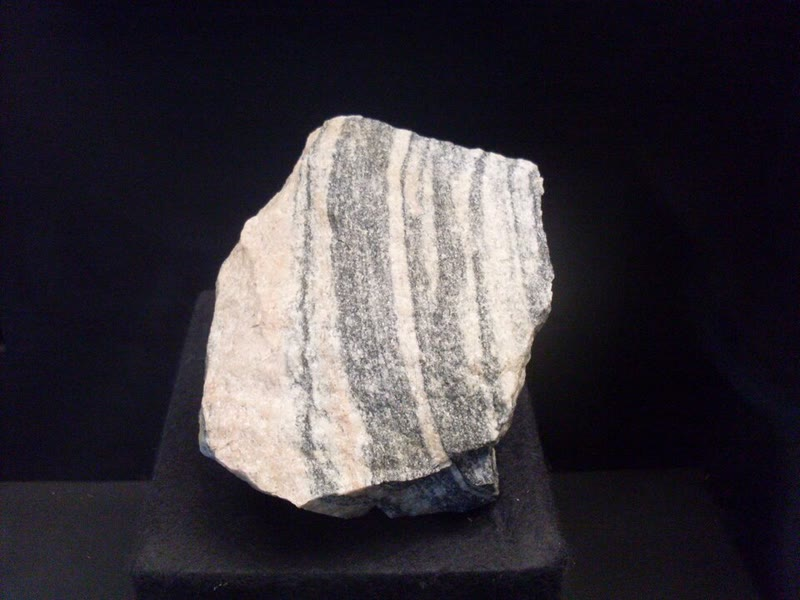
\includegraphics[height=4.6cm]{images/book2/g12-pedro-acasta-gneiss.jpg}\hspace{0.04\linewidth}%
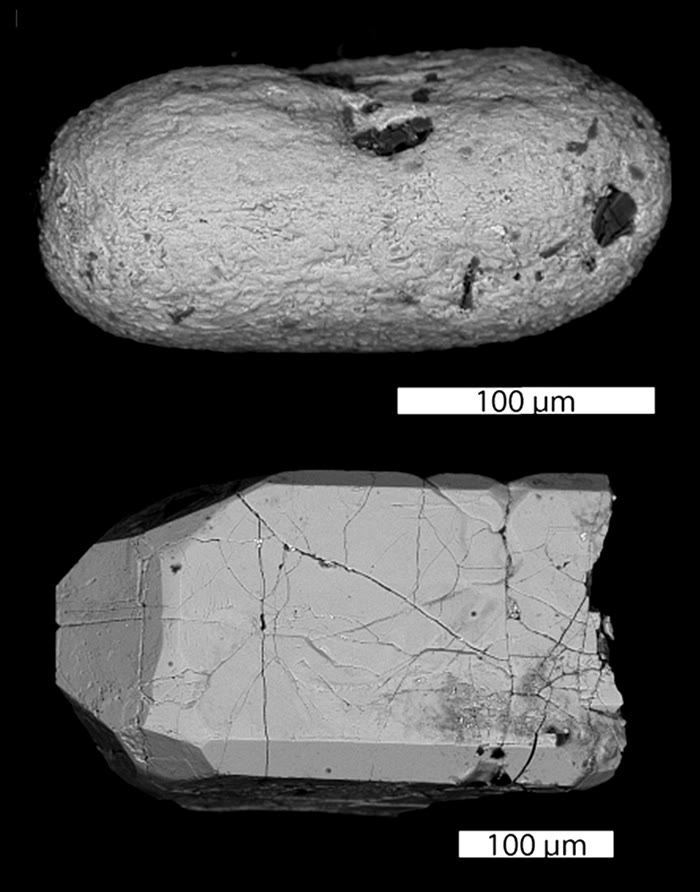
\includegraphics[height=4.6cm]{images/book2/g12-cavosie-jack-hills-zircons.jpg}

{\small Left: a piece of the Acasta gneiss, 4.03 billion years old, in a
museum display. Photograph Pedroalexandrade (CC~BY-SA~3.0). Right: two
zircon grains from the Jack Hills, Western Australia, seen with an electron
microscope; each scale bar is \qty{100}{\micro m}. The upper grain was
rounded as it was carried by water, the lower one kept its crystal faces.
Images A.~Cavosie and J.~Valley (public domain).}
\end{omfigure}
% ledger: photo:g12-acasta, photo:g12-jack-hills-zircons

\begin{recall}
The crust ends at the \omterm{def:g11:seismic-structure:moho}{Moho}, below which lies the denser mantle
(\cref{ch:g11:seismic-structure}). The \omterm{def:g11:ocean-ridges:oceanic-lithosphere}{oceanic crust} is about \qty{7}{km} of
basalt and \omterm{def:g11:ocean-ridges:gabbro}{gabbro} made at the ridges (\cref{ch:g11:ocean-ridges}), and it is
never older than about 190 million years (\cref{ch:g11:drift-to-spreading}).
The outer layers float on the \omterm{def:g11:lithosphere-asthenosphere:lithosphere}{asthenosphere}: in Airy's model, a region that
stands a height $h$ higher has a crust thicker by $h\,\rho_m/(\rho_m -
\rho_c)$ (\cref{ch:g11:lithosphere-asthenosphere}). Igneous rocks are named
by their \omterm{def:g11:igneous-rocks:texture}{texture} and their silica content: \omterm{def:g11:igneous-rocks:felsic-mafic}{mafic} from 45 to
\qty{55}{\percent} \ce{SiO2}, \omterm{def:g11:igneous-rocks:felsic-mafic}{intermediate} from 55 to 65, \omterm{def:g11:igneous-rocks:felsic-mafic}{felsic} from 65 to
75 (\cref{ch:g11:igneous-rocks}). Radioactive elements decay at a steady
rate, which gives rocks their ages (the physics books;
\cref{ch:g12:age-of-the-earth}).
\end{recall}
% ledger: white92:crust, data:b2-seafloor-age, tulane:magma-types

\section{What the continents are made of}

\begin{definition}[Continental crust]\label{def:g12:continental-crust:continental-crust}
The \emph{continental crust}\index{continental crust} is the crust that
forms the continents, including the parts of them under shallow seas. It is
thick, of granitic composition on average in its upper part, light, and it
can be very old.
\end{definition}
% ledger: tulane:crust-types, tulane:roots, cogley84:continents

The continents are larger than the land. The edges of the \omterm{def:g12:continental-crust:continental-crust}{continental crust}
lie under the sea, on the continental shelves: mapped this way, the
\omterm{def:g12:continental-crust:continental-crust}{continental crust} covers \num{210}~million~\unit{km^2}, \qty{41}{\percent} of the
Earth's surface, of which almost a third, \qty{30.6}{\percent}, is
submerged. Counted with its submerged parts, the mean height of the
\omterm{def:g12:continental-crust:continental-crust}{continental crust} is only about \qty{120}{m} above sea level.
% ledger: cogley84:continents

At the surface, the continents show every kind of rock --- sediments,
\omterm{def:g11:igneous-rocks:volcanic-plutonic}{volcanic rocks}, metamorphic rocks --- but beneath the sedimentary cover the
\omterm{def:g12:continental-crust:continental-crust}{continental crust} is made mostly of granitic rocks and of the metamorphic
and \omterm{def:g11:igneous-rocks:volcanic-plutonic}{plutonic rocks} of old mountain \omterm{def:g12:continental-crust:root}{roots}. On average, the whole \omterm{def:g12:continental-crust:continental-crust}{continental
crust} holds \qty{60.6}{\percent} silica; its upper part is richer,
\qty{66.6}{\percent}, so its deeper part must be poorer.
% ledger: rg14:crust, tulane:crust-types, cm95:crust

\begin{omfigure}
\begin{tikzpicture}
\begin{axis}[omrecord, ybar=0pt, width=0.92\linewidth, height=5.0cm, bar width=7pt,
  ymin=0, ymax=80, ylabel={mass fraction (\unit{\percent})},
  symbolic x coords={SiO2, Al2O3, FeO, MgO, CaO, Na2O, K2O},
  xticklabels={\ce{SiO2}, \ce{Al2O3}, \ce{FeO}, \ce{MgO}, \ce{CaO}, \ce{Na2O}, \ce{K2O}},
  xtick=data, enlarge x limits=0.08, ymajorgrids=true, xmajorgrids=false,
  legend style={font=\scriptsize, at={(0.98,0.97)}, anchor=north east, legend columns=1}]
% ledger: rg14:crust (upper and bulk continental crust; FeO* total iron)
\addplot[fill=omLithGranite, draw=black!60] coordinates {(SiO2,66.6) (Al2O3,15.4) (FeO,5.04) (MgO,2.48) (CaO,3.59) (Na2O,3.27) (K2O,2.80)};
\addplot[fill=omProp!55, draw=black!60] coordinates {(SiO2,60.6) (Al2O3,15.9) (FeO,6.71) (MgO,4.66) (CaO,6.41) (Na2O,3.07) (K2O,1.81)};
% ledger: earle:magma-oxides (mafic magma: midpoint of each range, the bar spans the range)
\addplot[fill=omLithBasalt, draw=black!60, error bars/.cd, y dir=both, y explicit]
  coordinates {(SiO2,50) +- (0,5) (Al2O3,16) +- (0,2) (FeO,10) +- (0,2) (MgO,7) +- (0,2) (CaO,9) +- (0,2) (Na2O,2) +- (0,1) (K2O,1.75) +- (0,1.25)};
\legend{upper continental crust, whole continental crust, mafic magma (range)}
\end{axis}
\end{tikzpicture}

{\small Composition of the \omterm{def:g12:continental-crust:continental-crust}{continental crust} compared with a \omterm{def:g11:igneous-rocks:felsic-mafic}{mafic} magma, the
kind that makes the \omterm{def:g11:ocean-ridges:oceanic-lithosphere}{oceanic crust}: the main oxides, in percent of the mass
(\ce{FeO} counts all the iron). The \omterm{def:g12:continental-crust:continental-crust}{continental crust} is richer in silica,
sodium and potassium, poorer in iron, magnesium and calcium. Data: Rudnick
and Gao (2014); \omterm{def:g11:igneous-rocks:felsic-mafic}{mafic} range from S.~Earle, \emph{Physical Geology}
(CC~BY~4.0).}
\end{omfigure}
% ledger: rg14:crust, earle:magma-oxides

\section{A thick, light crust}

Seismic surveys find the \omterm{def:g11:seismic-structure:moho}{Moho} beneath the continents at very different
depths. Averaged over all continents, weighted by area, the crust is about
\qty{41}{km} thick; it is thinner, about \qty{30}{km}, where the crust has
been stretched, and thicker, about \qty{46}{km} on average, in mountain belts.
Away from mountain belts it is commonly 35 to \qty{40}{km} thick; under the
highest ranges, 50 to \qty{70}{km}, about \qty{70}{km} under parts of Tibet.
The \omterm{def:g11:ocean-ridges:oceanic-lithosphere}{oceanic crust} is about \qty{7}{km} thick: the \omterm{def:g12:continental-crust:continental-crust}{continental crust} is five
to ten times thicker.
% ledger: cm95:crust, tulane:roots, karplus:tibet-moho, white92:crust

\begin{omfigure}
\begin{tikzpicture}
\begin{axis}[omrecord, xbar, bar shift=0pt, width=0.78\linewidth, height=5.0cm, bar width=8pt,
  xmin=0, xmax=80, ymin=0.4, ymax=5.6, ytick={1,...,5},
  yticklabels={oceanic crust, stretched continents, continents (average), mountain belts (average), under Tibet},
  xlabel={thickness of the crust (\unit{km})}, ymajorgrids=false,
  nodes near coords, nodes near coords style={font=\scriptsize, anchor=west}, point meta=explicit symbolic]
% ledger: white92:crust, cm95:crust, karplus:tibet-moho
\addplot[fill=omLithBasalt, draw=black!60] coordinates {(7.1,1) [7.1]};
\addplot[fill=omLithGranite, draw=black!60] coordinates {(30.5,2) [30.5] (41.1,3) [41.1] (46.3,4) [46.3] (70,5) [about 70]};
\end{axis}
\end{tikzpicture}

{\small Thickness of the crust from seismic measurements. Data: White,
McKenzie and O'Nions (1992) for the \omterm{def:g11:ocean-ridges:oceanic-lithosphere}{oceanic crust}; Christensen and Mooney
(1995) for the continental averages; Karplus and others (2019) for Tibet.}
\end{omfigure}
% ledger: white92:crust, cm95:crust, karplus:tibet-moho

The \omterm{def:g12:continental-crust:continental-crust}{continental crust} is also light. Its mean density is about
\qty{2830}{kg/m^3}. The basalt and \omterm{def:g11:ocean-ridges:gabbro}{gabbro} of the \omterm{def:g11:ocean-ridges:oceanic-lithosphere}{oceanic crust}, rich in
pyroxene and olivine, come to about \qty{3000}{kg/m^3}
(\cref{ch:g11:minerals}), and the mantle just beneath the \omterm{def:g11:seismic-structure:moho}{Moho} to about
\qty{3380}{kg/m^3}. A thick and light crust floats high: this is why the
continents stand above the ocean floor, and why a continent cannot be dragged
down at a \omterm{def:g11:subduction-zones:subduction}{subduction zone}. Where a continent arrives at a trench, it is too
light to sink; \omterm{def:g11:subduction-zones:subduction}{subduction} stops, and the two continents collide
(\cref{ch:g12:mountain-building}). \omterm{def:g12:continental-crust:continental-crust}{Continental crust}, once made, is hard to
destroy.
% ledger: cm95:crust, data:prem, tulane:roots, tulane:no-subduct
% values (mineral_density.py): basalt/gabbro rock line 3.0015 g/cm3

\begin{omfigure}
\begin{tikzpicture}[x=1cm, y=0.075cm, font=\footnotesize]
  % continental column: 41 km of crust, surface at +0.12 km (mean height); ocean column: 3.7 km of water drawn schematically
  \fill[omLithGranite] (0,0) rectangle (3,-41);
  \fill[omLithPeridotite!60] (0,-41) rectangle (3,-60);
  \fill[omSea] (6,0) rectangle (9,-4);
  \fill[omLithGabbro] (6,-4) rectangle (9,-11.1);
  \fill[omLithPeridotite!60] (6,-11.1) rectangle (9,-60);
  \draw[black!60] (0,0) rectangle (3,-60) (6,0) rectangle (9,-60);
  \draw[line width=0.9pt] (0,-41) -- (3,-41) (6,-11.1) -- (9,-11.1);
  \node[align=center] at (1.5,-20) {continental crust\\about \qty{41}{km}\\\qty{2830}{kg/m^3}\\up to 4 billion years};
  \node[align=center] at (7.5,-24) {mantle\\\qty{3380}{kg/m^3}\\below the Moho};
  \node[align=center] at (1.5,-50.5) {mantle};
  \node at (7.5,-2) {ocean};
  \draw[black!60] (8.6,-7.6) -- (9.3,-7.6);
  \node[anchor=west, align=left] at (9.3,-7.6) {oceanic crust, about \qty{7}{km}\\\qty{3000}{kg/m^3}\\less than 200 million years};
  \node[anchor=east] at (-0.1,-41) {Moho};
  \node[anchor=east] at (5.9,-11.1) {Moho};
  \node[anchor=south] at (1.5,0) {a continent};
  \node[anchor=south] at (7.5,0) {an ocean};
  \foreach \d in {0,20,40,60} {\draw[black!60] (-1.5,-\d) -- (-1.3,-\d); \node[anchor=east, font=\scriptsize] at (-1.5,-\d) {\d};}
  \draw[black!60] (-1.4,0) -- (-1.4,-60);
  \node[rotate=90, font=\scriptsize] at (-2.3,-30) {depth (\unit{km})};
\end{tikzpicture}

{\small A continent and an ocean side by side (depths to scale, widths not;
the ocean drawn \qty{4}{km} deep): the \omterm{def:g12:continental-crust:continental-crust}{continental crust} is thicker, lighter
and much older than the \omterm{def:g11:ocean-ridges:oceanic-lithosphere}{oceanic crust}.}
\end{omfigure}
% ledger: cm95:crust, white92:crust, data:prem, bowring99:acasta, data:b2-seafloor-age

\begin{method}[Comparing continental and oceanic crust]\label{met:g12:continental-crust:compare}
To tell which kind of crust lies under a place, compare five properties:
\begin{enumerate}
  \item the thickness: about \qty{7}{km} for \omterm{def:g11:ocean-ridges:oceanic-lithosphere}{oceanic crust}, 30 to
        \qty{70}{km} for \omterm{def:g12:continental-crust:continental-crust}{continental crust};
  \item the rocks: basalt and \omterm{def:g11:ocean-ridges:gabbro}{gabbro}, or granite, gneiss and their
        relatives, under a cover of sediments;
  \item the composition: about \qty{50}{\percent} silica, or about 60 and
        more;
  \item the density: about \qty{3000}{kg/m^3}, or about \qty{2830}{kg/m^3};
  \item the age: less than 200 million years, or up to 4 billion years.
\end{enumerate}
The elevation is a clue, not a test: most of the ocean floor lies
kilometres deep, but the edges of the continents lie under shallow seas.
\end{method}
% ledger: white92:crust, cm95:crust, rg14:crust, earle:magma-oxides, cogley84:continents

\begin{example}[A shallow sea floor]\label{ex:g12:continental-crust:shelf}
A survey ship finds a sea floor \qty{150}{m} deep. Seismic profiles put the
\omterm{def:g11:seismic-structure:moho}{Moho} \qty{32}{km} below the sea floor; a drill core brings up, under the
sediments, a coarse-grained rock of quartz, feldspar and mica. Which crust
lies there?

\emph{Solution.} Thickness about \qty{32}{km}: continental, thinner than
average, as where it has been stretched. A granite under the sediments:
continental. The sea floor is a continental shelf, one of the submerged
parts that make up almost a third of the continents.
\end{example}
% invented numbers; ledger: cm95:crust, cogley84:continents

How heavy is all this crust? A layer that is thin compared with the Earth's
radius has a simple mass.

\begin{proposition}[The mass of a thin layer]\label{prop:g12:continental-crust:thin-layer}
A layer of thickness $H$ and density $\rho$ covering a fraction $f$ of the
surface of a planet of radius $R \gg H$ and mean density $\bar\rho$ has a
mass $m \approx 4\pi R^2 f H \rho$, and its share of the planet's mass $M$ is
\[
  \frac{m}{M} \approx 3 f\,\frac{H}{R}\,\frac{\rho}{\bar\rho}.
\]
\end{proposition}
% ledger: earth:Rmean, earth:density

\begin{proof}
The surface of the planet is $4\pi R^2$; the layer covers $4\pi R^2 f$ and,
being thin, has a volume close to that area times $H$, so $m \approx 4\pi R^2
f H \rho$. The planet's mass is $M = \tfrac{4}{3}\pi R^3 \bar\rho$. Dividing,
$m/M \approx 4\pi R^2 f H \rho / (\tfrac{4}{3}\pi R^3 \bar\rho) = 3 f (H/R)
(\rho/\bar\rho)$.
\end{proof}

For the \omterm{def:g11:ocean-ridges:oceanic-lithosphere}{oceanic crust} --- the remaining \qty{59}{\percent} of the surface,
\qty{7.1}{km}, about \qty{3000}{kg/m^3} --- with $R = \qty{6371}{km}$ and
$\bar\rho = \qty{5513}{kg/m^3}$, the share is $3 \times 0.59 \times
(7.1/6371) \times (3000/5513) \approx 0.0011$: about a tenth of a percent of
the Earth's mass. The weekend problem does the same for the continents.
% ledger: cogley84:continents, white92:crust, earth:Rmean, earth:density

\section{An old crust}

The ocean floor is young everywhere: three quarters of it is younger than
100 million years, and almost none older than 190 million years. The
continents are another matter. Their rocks span almost the whole history of
the Earth, from the Acasta gneiss, 4.03 billion years old, to lavas erupted
today, and grains of zircon carry the record back to 4.4 billion years.
% ledger: data:b2-seafloor-age, bowring99:acasta, uw14:jack-hills

\begin{omfigure}
\begin{tikzpicture}
\begin{axis}[omrecord, ybar interval, width=0.82\linewidth, height=5.0cm,
  xmin=0, xmax=200, ymin=0, ymax=0.12, xtick={0,20,...,200},
  xlabel={age of the ocean floor (millions of years)},
  ylabel={share of the ocean floor}, yticklabel style={/pgf/number format/fixed},
  ymajorgrids=true, xmajorgrids=false, clip=false, x tick label as interval=false]
% computed in figdata/grade-12/crust_ages.py (Seton 2020 grid, 1-degree cells, area-weighted)
\addplot[fill=omDef!35, draw=omDef] table[x=age_lo, y=share] {figdata/out/grade-12-crust_ages-hist.dat};
\node[anchor=north east, align=right, font=\scriptsize, fill=white, inner sep=2pt] at (axis cs:198,0.115)
  {oldest continental rock: \num{4030} million years,\\twenty times older than the oldest ocean floor};
\end{axis}
\end{tikzpicture}

{\small How old the ocean floor is: the share of its area in each band of 10
million years. The young floor dominates; almost nothing is older than 190
million years (a few old basins of the eastern Mediterranean are left out).
Data: Seton and others (2020), computed.}
\end{omfigure}
% ledger: data:b2-seafloor-age, bowring99:acasta
% values (crust_ages.py): oldest_open_myr 192.5, share_younger_100 0.765, share_younger_150 0.956, rock_over_floor 20.9

The oldest parts of the continents form their cores.

\begin{definition}[Craton]\label{def:g12:continental-crust:craton}
A \emph{craton}\index{craton} is an old and stable core of a continent:
\omterm{def:g12:continental-crust:continental-crust}{continental crust} formed and deformed more than a billion years ago, which
has since cooled and no longer deforms. Its rocks are mostly metamorphic and
\omterm{def:g11:igneous-rocks:volcanic-plutonic}{plutonic rocks}, the deep \omterm{def:g12:continental-crust:root}{roots} of former mountains.
\end{definition}
% ledger: tulane:cratons

Around the \omterm{def:g12:continental-crust:craton}{cratons} lie belts of younger deformed rocks, the eroded \omterm{def:g12:continental-crust:root}{roots} of
mountain ranges built later; the belts tend to be younger towards the edges
of a continent. A continent has grown by mountain building that welded new
crust to its edges, around an ancient core. In Canada, where the \omterm{def:g12:continental-crust:craton}{craton}'s
rocks lie at the surface, gneisses and granites 1 to 3 billion years old crop
out, here on a lakeshore.
% ledger: tulane:cratons, photo:g12-canadian-shield

\begin{omfigure}
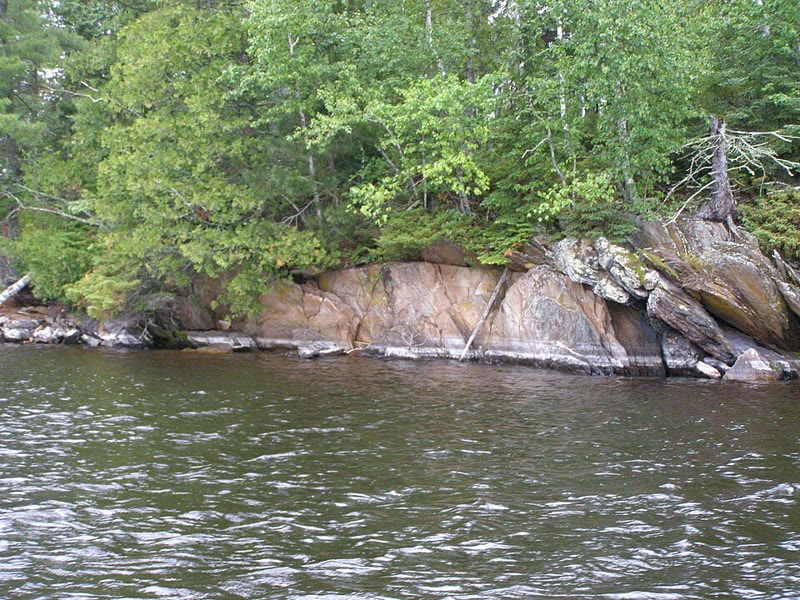
\includegraphics[height=5.0cm]{images/book2/g12-light-canadian-shield.jpg}

{\small Gneisses and granites 1 to 3 billion years old on a lakeshore in
Canada, part of the ancient core of North America. Photograph Chris Light
(CC~BY-SA~4.0).}
\end{omfigure}
% ledger: photo:g12-canadian-shield

Why does the \omterm{def:g12:continental-crust:continental-crust}{continental crust} last, while the ocean floor is always young?
The \omterm{def:g11:ocean-ridges:oceanic-lithosphere}{oceanic crust} is dense: it sinks back into the mantle at \omterm{def:g11:subduction-zones:subduction}{subduction zones},
and none of it survives much more than 200 million years. The \omterm{def:g12:continental-crust:continental-crust}{continental
crust} is too light to sink; it can be worn down by erosion, stretched or
crumpled, but it stays at the surface. The rocks of a continent are an
archive of four billion years.
% ledger: tulane:no-subduct, tulane:roots, data:b2-seafloor-age

\section{Mountain roots}

The higher the mountains, the thicker the crust beneath them.

\begin{definition}[Mountain root]\label{def:g12:continental-crust:root}
The \emph{root}\index{root (of a mountain range)} of a mountain range is
the part of its thickened crust that reaches down into the mantle below the
level of the \omterm{def:g11:seismic-structure:moho}{Moho} beneath the surrounding lowlands.
\end{definition}
% ledger: tulane:roots

Airy's model predicts the \omterm{def:g12:continental-crust:root}{root}: a range standing $h$ above its
surroundings has a \omterm{def:g12:continental-crust:root}{root} $r = h\,\rho_c/(\rho_m - \rho_c)$, about five times
its height with $\rho_c = \qty{2830}{kg/m^3}$ and $\rho_m =
\qty{3380}{kg/m^3}$ (\cref{prop:g11:lithosphere-asthenosphere:airy}). Two
kinds of measurements see the \omterm{def:g12:continental-crust:root}{roots}. Seismic surveys find the \omterm{def:g11:seismic-structure:moho}{Moho} deeper
under ranges: 50 to \qty{70}{km} under many mountain belts, about
\qty{70}{km} under parts of Tibet. Gravity is weaker over mountain ranges than
their visible mass would suggest: the light \omterm{def:g12:continental-crust:root}{root}, standing in place of
denser mantle, makes up a deficit of mass at depth, and the measured gravity
anomalies follow the topography and the thickness of the crust found by
seismology. The continents float, and their mountains float highest.
% ledger: tulane:roots, karplus:tibet-moho, cm95:crust, data:prem

\section{Exercises}

\begin{exercise}[$\star$]\label{exo:g12:continental-crust:1}
Copy and complete for the continental and the \omterm{def:g11:ocean-ridges:oceanic-lithosphere}{oceanic crust}: thickness;
main rocks; silica content; density; greatest age.
\end{exercise}

\begin{exercise}[$\star$]\label{exo:g12:continental-crust:2}
The whole \omterm{def:g12:continental-crust:continental-crust}{continental crust} holds \qty{60.6}{\percent} silica, its upper
part \qty{66.6}{\percent}. Using the silica classes of igneous rocks, is
each \omterm{def:g11:igneous-rocks:felsic-mafic}{mafic}, \omterm{def:g11:igneous-rocks:felsic-mafic}{intermediate} or \omterm{def:g11:igneous-rocks:felsic-mafic}{felsic}? Name a \omterm{def:g11:igneous-rocks:volcanic-plutonic}{plutonic rock} of the same
composition.
\end{exercise}

\begin{exercise}[$\star$]\label{exo:g12:continental-crust:3}
Why can the \omterm{def:g11:ocean-ridges:oceanic-lithosphere}{oceanic crust} sink into the mantle at a \omterm{def:g11:subduction-zones:subduction}{subduction zone}, and not
the \omterm{def:g12:continental-crust:continental-crust}{continental crust}? Answer with densities.
\end{exercise}

\begin{exercise}[$\star$]\label{exo:g12:continental-crust:4}
(1) What is a \omterm{def:g12:continental-crust:craton}{craton}? (2) How old are the rocks of a \omterm{def:g12:continental-crust:craton}{craton} at least?
(3) Which kinds of rocks make it up?
\end{exercise}

\begin{exercise}[$\star$]\label{exo:g12:continental-crust:5}
The oldest ocean floor is about 190 million years old, the Acasta gneiss
4.03 billion years. How many times older is the gneiss? Why is there no
ocean floor as old?
\end{exercise}

\begin{exercise}[$\star\star$]\label{exo:g12:continental-crust:6}
The \omterm{def:g12:continental-crust:continental-crust}{continental crust} covers \num{210.4}~million~\unit{km^2}, of which
\qty{30.6}{\percent} is under the sea. (1) What area of \omterm{def:g12:continental-crust:continental-crust}{continental crust}
lies under the sea? (2) What area stands above it? (3) The Earth's surface is
$4\pi R^2$ with $R = \qty{6371}{km}$. What share of the surface does the
\omterm{def:g12:continental-crust:continental-crust}{continental crust} cover?
\end{exercise}

\begin{exercise}[$\star\star$]\label{exo:g12:continental-crust:7}
Compute the mass of a column of crust \qty{1}{m^2} in cross-section,
from the surface to the \omterm{def:g11:seismic-structure:moho}{Moho}: (1) through \qty{41.1}{km} of \omterm{def:g12:continental-crust:continental-crust}{continental
crust} at \qty{2830}{kg/m^3}; (2) through \qty{7.1}{km} of \omterm{def:g11:ocean-ridges:oceanic-lithosphere}{oceanic crust} at
\qty{3000}{kg/m^3}. (3) How many times heavier is the first?
\end{exercise}

\begin{exercise}[$\star\star$]\label{exo:g12:continental-crust:8}
A range stands \qty{2.5}{km} above lowlands whose crust is \qty{35}{km}
thick. With $\rho_c = \qty{2830}{kg/m^3}$ and $\rho_m =
\qty{3380}{kg/m^3}$, compute its \omterm{def:g12:continental-crust:root}{root} and the thickness of its crust. Is
the result in the range measured under mountain belts?
\end{exercise}

\begin{exercise}[$\star\star$]\label{exo:g12:continental-crust:9}
From the histogram of ocean-floor ages: (1) what share of the ocean floor is
younger than 30 million years? (2) Which band of 10 million years holds the
most floor? (3) Why does the share fall towards old ages?
\end{exercise}

\begin{exercise}[$\star\star$]\label{exo:g12:continental-crust:10}
Mapped with its submerged parts, the \omterm{def:g12:continental-crust:continental-crust}{continental crust} has a mean height of
about \qty{120}{m}. Suppose its submerged parts, \qty{30.6}{\percent} of its
area, lie on average \qty{100}{m} below sea level. What is the mean height of
its emerged part? Why do older estimates that counted only the land give a
much higher mean height?
\end{exercise}

\begin{exercise}[$\star\star$]\label{exo:g12:continental-crust:11}
A drill hole on an island far out in an ocean reaches, below a few hundred
metres of lavas, a \omterm{def:g11:ocean-ridges:gabbro}{gabbro}; seismic profiles put the \omterm{def:g11:seismic-structure:moho}{Moho} \qty{8}{km} down.
Another drill hole, under a broad, flat plain, reaches gneiss at \qty{2}{km},
and the \omterm{def:g11:seismic-structure:moho}{Moho} lies \qty{38}{km} down. Use the method to decide which crust
lies under each.
\end{exercise}

\begin{exercise}[$\star\star\star$]\label{exo:g12:continental-crust:12}
How good is the approximation of the proposition? (1) Compute the exact
volume of a shell of thickness \qty{41.1}{km} at the surface of a sphere of
radius \qty{6371}{km}, $\tfrac{4}{3}\pi\bigl(R^3 - (R - H)^3\bigr)$, and the
approximate one, $4\pi R^2 H$. (2) What is the relative difference? Compare
it with $H/R$.
\end{exercise}

\begin{exercise}[$\star\star\star$]\label{exo:g12:continental-crust:13}
Suppose the upper third of the \omterm{def:g12:continental-crust:continental-crust}{continental crust}, by mass, holds
\qty{66.6}{\percent} silica, and the whole crust \qty{60.6}{\percent}. (1)
What is the silica content of the lower two thirds? (2) Which class of
igneous rock does it match? (3) What does that say about the deep
\omterm{def:g12:continental-crust:continental-crust}{continental crust}?
\end{exercise}

\begin{exercise}[$\star\star\star$]\label{exo:g12:continental-crust:14}
Suppose that new \omterm{def:g11:ocean-ridges:oceanic-lithosphere}{oceanic crust} forms at the ridges at about \qty{3}{km^2} a
year, and that the ocean floor covers about \num{300}~million~\unit{km^2}. (1)
How long would the ridges take to make an area equal to the whole ocean
floor? (2) Compare with the ages of the ocean floor. (3) What must happen to
the old floor?
\end{exercise}

\begin{exercise}[$\star\star\star$]\label{exo:g12:continental-crust:15}
Suppose all the \omterm{def:g12:continental-crust:continental-crust}{continental crust}, \qty{8.6e9}{km^3}, had formed at a steady
rate since 4.0 billion years ago. (1) Compute the rate in cubic kilometres a
year. (2) The zircons of the Jack Hills show that some crust already existed
4.4 billion years ago. Does a steady rate fit a world in which most of the
crust might have formed early, or late? What could the oldest rocks tell, and
what can they not, given that old crust can be eroded or recycled?
\end{exercise}

\section{Problem: How Heavy Is the Continental Crust?}

\begin{problem}[{Weekend problem --- the mass of the continents}]
\label{pb:g12:continental-crust:1}
% ledger: cogley84:continents, cm95:crust, earth:mass, earth:Rmean, earth:density, white92:crust
% values: 4 pi R^2 = 5.1006e8 km2; V = 210.4e6 x 41.1 = 8.647e9 km3; m = 2.447e22 kg; m/M = 0.410 %
The \omterm{def:g12:continental-crust:continental-crust}{continental crust} covers \num{210.4}~million~\unit{km^2} (submerged parts
included). Seismic surveys give it an average thickness of \qty{41.1}{km} and
a mean density of \qty{2830}{kg/m^3}. The Earth has a mean radius of
\qty{6371}{km}, a mass of \qty{5.9722e24}{kg} and a mean density of
\qty{5513}{kg/m^3}.

\medskip
\noindent\textbf{Part I --- The area.}
\begin{enumerate}
  \item Compute the area of the Earth's surface, $4\pi R^2$, in
        \unit{km^2}.
  \item What share of it does the \omterm{def:g12:continental-crust:continental-crust}{continental crust} cover?
  \item \qty{30.6}{\percent} of the \omterm{def:g12:continental-crust:continental-crust}{continental crust} lies under the sea.
        What area is that?
  \item What area of the Earth's surface is left for the \omterm{def:g11:ocean-ridges:oceanic-lithosphere}{oceanic crust},
        assuming the rest is all oceanic?
  \item Why is the \omterm{def:g12:continental-crust:continental-crust}{continental crust} larger than the land?
\end{enumerate}

\medskip
\noindent\textbf{Part II --- Thickness and volume.}
\begin{enumerate}[resume]
  \item Why can the volume be computed as area times thickness, though the
        crust lies on a sphere?
  \item Compute the volume of the \omterm{def:g12:continental-crust:continental-crust}{continental crust} in \unit{km^3}.
  \item Convert it to \unit{m^3}.
  \item Another estimate of the average thickness is \qty{36}{km}. What
        volume does it give?
  \item By how much, in percent, do the two volumes differ?
\end{enumerate}

\medskip
\noindent\textbf{Part III --- Density and mass.}
\begin{enumerate}[resume]
  \item Compute the mass of the \omterm{def:g12:continental-crust:continental-crust}{continental crust} with \qty{41.1}{km}.
  \item Compute the mass of a \qty{1}{m^2} column through the \omterm{def:g12:continental-crust:continental-crust}{continental
        crust}.
  \item Compute the mass of the \omterm{def:g11:ocean-ridges:oceanic-lithosphere}{oceanic crust}: area from question~4,
        thickness \qty{7.1}{km}, density \qty{3000}{kg/m^3}.
  \item Which is heavier, and by how many times? Why, though it covers less
        area?
  \item Why is the \omterm{def:g12:continental-crust:continental-crust}{continental crust} less dense than the \omterm{def:g11:ocean-ridges:oceanic-lithosphere}{oceanic crust}?
\end{enumerate}

\medskip
\noindent\textbf{Part IV --- Compared with the Earth.}
\begin{enumerate}[resume]
  \item Divide the mass of question~11 by the Earth's mass.
  \item Check the result with the proposition on thin layers.
  \item What share of the Earth's mass is the \omterm{def:g11:ocean-ridges:oceanic-lithosphere}{oceanic crust}?
  \item The \omterm{def:g12:continental-crust:continental-crust}{continental crust} holds the only rocks older than about 200
        million years. What share of the Earth's mass carries the record of
        almost all of its history?
  \item Conclude: what share of the Earth's mass is the \omterm{def:g12:continental-crust:continental-crust}{continental crust}?
\end{enumerate}
\end{problem}
